\section{Streaming Pipeline}
\label{sec:system}

The experiments run on the \mosaic pipeline~\cite{mosaic2026}, extended
for this study. It has two transport stages (Figure~\ref{fig:architecture},
Table~\ref{tab:testbed}). Stage~1 delivers encoded \vpcc content from
the origin server to an edge renderer over \quic and is where
impairment is injected. Stage~2 casts the rendered stereo frames from
the edge renderer to the \hmd over a private \fiveg standalone network
and is identical across conditions, so any variation in perceived
quality originates in Stage~1. This section describes the components
in full, including those that the conference version could only
summarise: content preparation (Section~\ref{sec:sys-content}), origin
and impairment (Section~\ref{sec:sys-stage1}), edge decoding and
rendering (Section~\ref{sec:sys-edge}) and \fiveg access for the
headset (Section~\ref{sec:sys-stage2}).

\begin{figure*}[t]
  \centering
  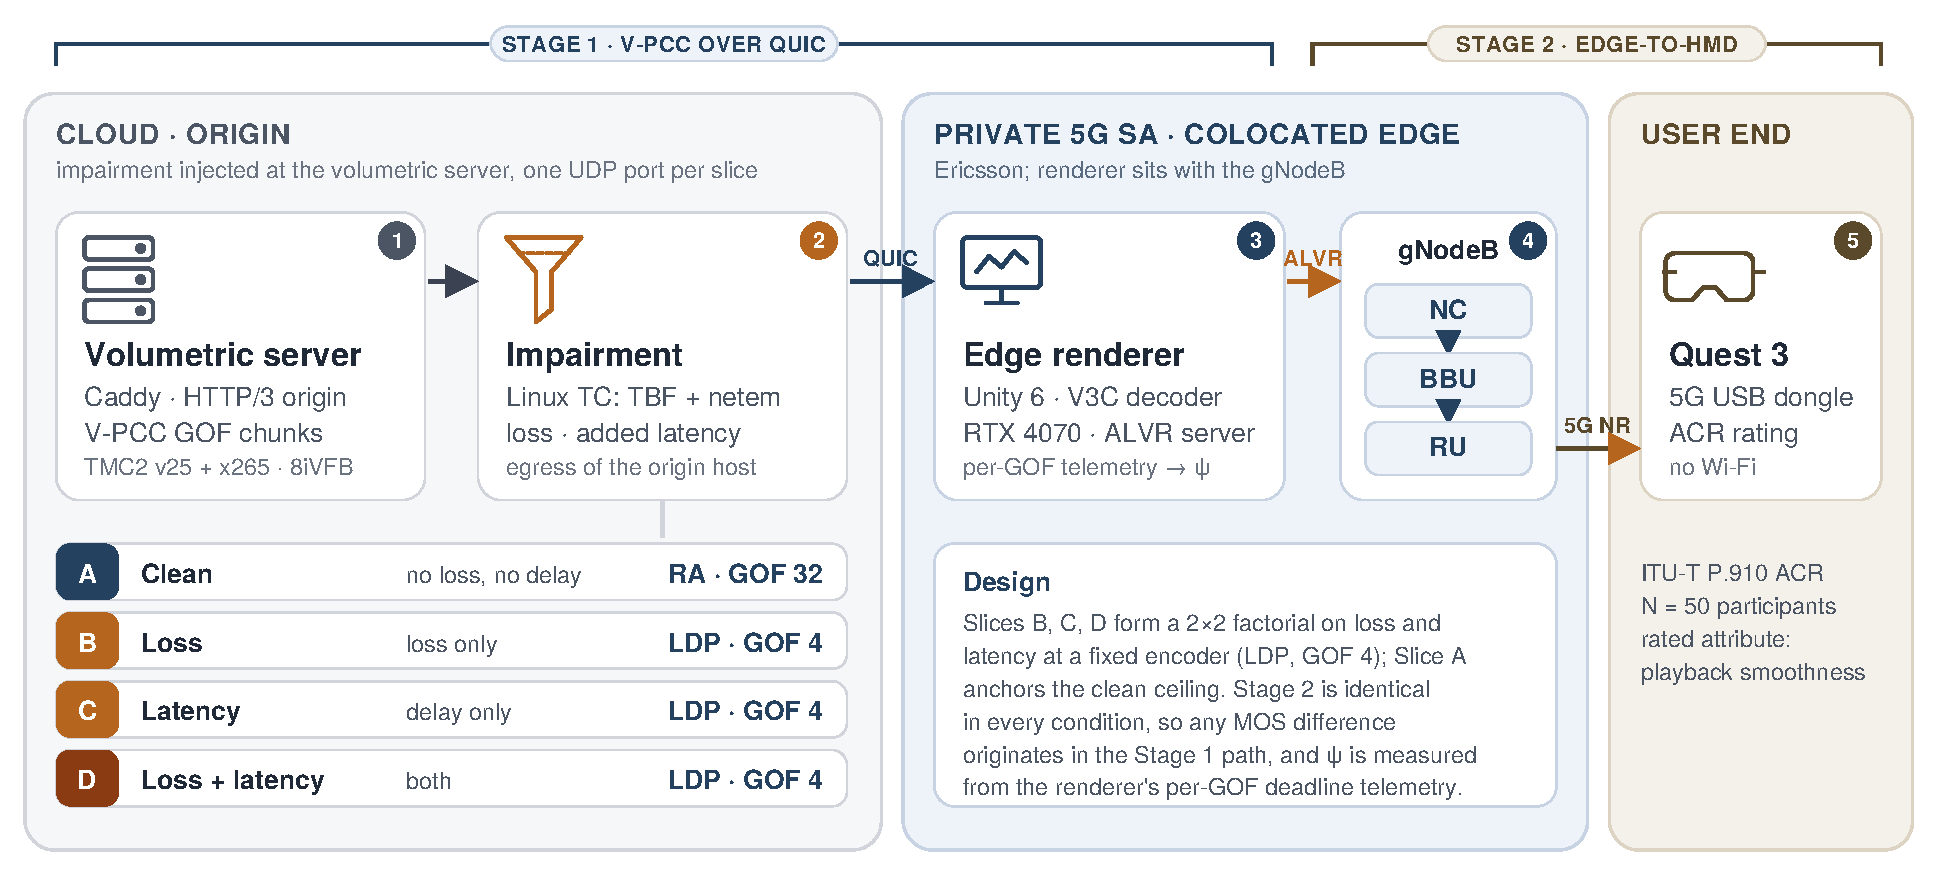
\includegraphics[width=\textwidth]{pipeline.pdf}
  \caption{End-to-end pipeline. Stage~1 delivers \vpcc content from the
  volumetric server~\ding{172}, where impairment is injected at the
  host's egress on one UDP port per slice~\ding{173}, over reliable
  \quic to the edge renderer~\ding{174}, colocated with the
  gNodeB~\ding{175} of the private \fiveg network. Stage~2 casts the
  rendered stereo frames through the network controller, baseband unit
  and radio unit to the Meta Quest~3~\ding{176} and is identical across
  conditions.}
  \label{fig:architecture}
\end{figure*}

\begin{table}[t]
  \caption{Testbed components.}
  \label{tab:testbed}
  \centering
  \small
  \begin{tabular}{@{}ll@{}}
    \toprule
    Component & Specification \\
    \midrule
    Volumetric server & Ubuntu 24.04, Caddy v2.11 (quic-go), HTTP/3, TLS~1.3 AES-128-GCM \\
    Impairment        & Linux TC (TBF + netem chain), one UDP port per slice \\
    Edge renderer     & Windows~11, NVIDIA RTX~4070, Unity~6, 5G-MAG V3C native decoder \\
    Presentation      & Native OpenGL$\to$DX11 interop plugin, SteamVR, ALVR \\
    5G network        & Ericsson private 5G SA, edge colocated with the gNodeB \\
    \hmd              & Meta Quest~3 (Snapdragon XR2 Gen~2), adapted 5G USB dongle \\
    \bottomrule
  \end{tabular}
\end{table}

\subsection{Content Preparation}
\label{sec:sys-content}

\paragraph{Sequences.}
Three sequences of the 8i Voxelized Full Bodies dataset~\cite{8i},
Category~2 of the \vpcc common test conditions~\cite{vpccctc}, are used
(Figure~\ref{fig:content}): Longdress (vox10, $\approx$0.85\,M
points/frame), Soldier (vox10, $\approx$1.08\,M) and ThaiDancer (vox12,
$\approx$3.13\,M). Each is \SI{10}{\second} long, 300 frames at
\SI{30}{fps}, and depicts a single person in motion.

\begin{figure}[t]
  \centering
  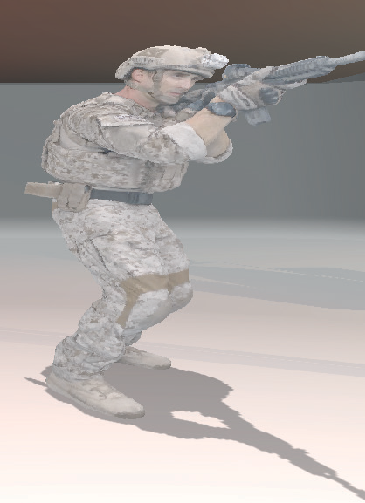
\includegraphics[height=2.6cm]{view-sd-front.pdf}\hfill
  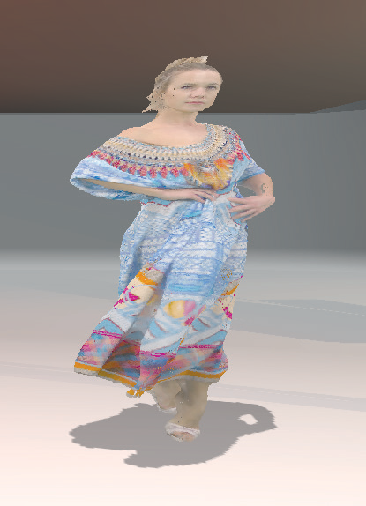
\includegraphics[height=2.6cm]{view-ld-front.pdf}\hfill
  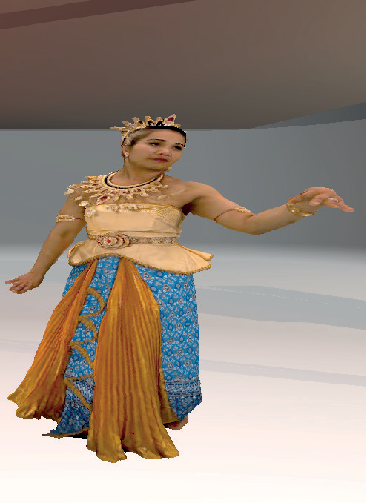
\includegraphics[height=2.6cm]{view-td-front.pdf}\hfill
  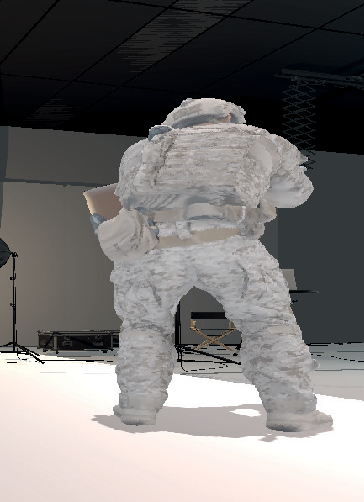
\includegraphics[height=2.6cm]{view-sd-back.pdf}\hfill
  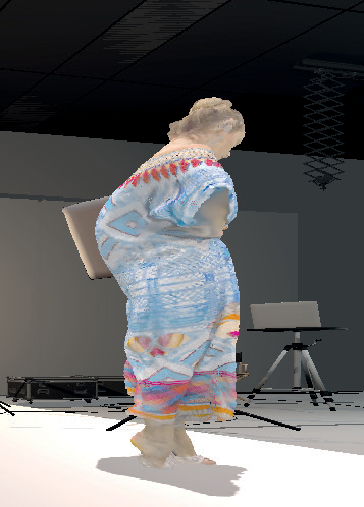
\includegraphics[height=2.6cm]{view-ld-back.pdf}\hfill
  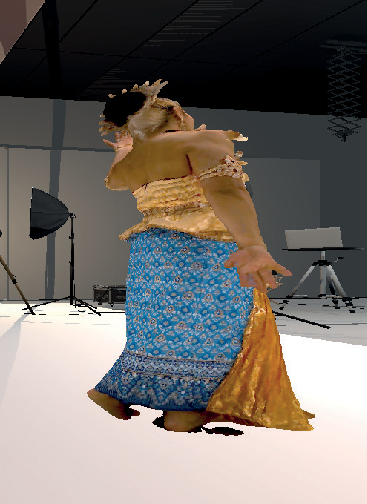
\includegraphics[height=2.6cm]{view-td-back.pdf}
  \caption{Soldier, Longdress and ThaiDancer in the rendering scene,
  front (first three) and back (last three) views.}
  \label{fig:content}
\end{figure}

\paragraph{Encoder.}
\gls{tmc2}~v25~\cite{tmc2} is the \vpcc reference software, but its
encoding time is dominated by the \gls{hevc} reference encoder
\gls{hm}, which codes the occupancy, geometry and attribute videos
separately. We replace \gls{hm} for the geometry and attribute videos
with x265~\cite{x265} through a command-line shim that accepts
\gls{hm}'s interface and dispatches FFmpeg~6.1 with libx265, so that
\gls{tmc2} runs unmodified and unaware of the substitution. The
\gls{ldp} configurations use \texttt{bframes=0},
\texttt{tune=zerolatency} and \texttt{preset=fast}; the \gls{ra}
configuration uses \texttt{bframes=15} and \texttt{preset=medium}.
Occupancy maps, which are coded losslessly, remain with \gls{hm}. With
the shim, one configuration of a vox10 sequence encodes in
\SIrange{25}{30}{\minute} and of the vox12 sequence in
\SIrange{110}{120}{\minute} on a single workstation, which makes a
multi-configuration sweep tractable.

The patch packer of \gls{tmc2} may change atlas dimensions within a
sequence, and the real-time decoder of Section~\ref{sec:sys-edge} does
not support such a change mid-stream. Atlas dimensions are therefore
fixed per sequence and configuration with \gls{tmc2}'s minimum image
width and height options (a minimum height of 4096 for ThaiDancer).

\paragraph{Encoding campaign.}
Each sequence is encoded in three configurations that differ in
prediction structure and \gof length: \gls{ra} with a hierarchical
I/P/B structure and a \gof of 32, as prescribed by the \vpcc common
test conditions~\cite{vpccctc}, and \gls{ldp} with I- and P-frames
only~\cite{hmctc} and \gofs of 16 and 4. Geometry QP (16) and occupancy
precision (2) are fixed and the attribute QP is swept.
Figure~\ref{fig:rd} reports the resulting rate--distortion curves of
the attribute video. Two observations guide the operating points. The
gap between sequences at a fixed bitrate (about \SI{4}{dB}) is an
order of magnitude larger than the gap between configurations of the
same sequence (\SIrange{0.3}{0.6}{dB}), so differences between contents
cannot be removed by encoder tuning; and \gls{ra} lies on or just
above the \gls{ldp} curves, so the shorter \gls{ldp} \gofs trade coding
efficiency for resilience to transport delay rather than for fidelity.
The attribute QPs selected (Table~\ref{tab:encoder}) give a
\gls{psnr}$_Y$ between 34 and \SI{39}{dB} and place all three sequences
in a common bitrate band (shaded), so that differences across
conditions are attributable to transport and content rather than to
bitrate. Attribute data dominate the bitstream: for Longdress,
attribute coding accounts for about 92\% of the encoded size, geometry
for 6\% and occupancy for 1\%. \pcqm~\cite{pcqm} is computed per
sequence as a stimulus descriptor and does not enter the model
(Section~\ref{sec:model-scope}).

\begin{figure}[t]
  \centering
  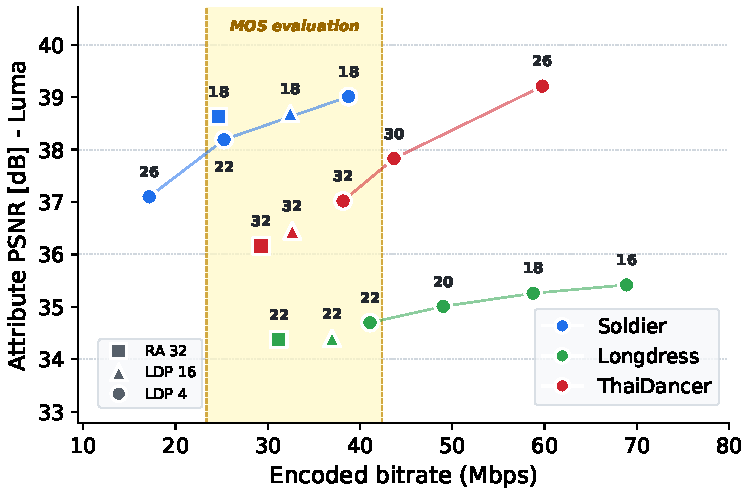
\includegraphics[width=0.62\linewidth]{rate-distortion.pdf}
  \caption{Rate--distortion curves of the attribute video for the three
  encoder configurations; labels are attribute QPs. The shaded band
  marks the bitrate range of the encoded sequences used in the
  subjective studies.}
  \label{fig:rd}
\end{figure}

\paragraph{Delivery units.}
Each bitstream is split into one object per \gof with the
VpccChunkCreator tool of the 5G-MAG platform~\cite{fivegmag}: a
300-frame sequence yields 75 objects of \SI{133}{\milli\second} at
\gls{ldp} \gof{}=4, 19 of \SI{533}{\milli\second} at \gls{ldp} \gof{}=16
and 10 of \SI{1067}{\milli\second} at \gls{ra} \gof{}=32. These objects
are the delivery units $k$ of Section~\ref{sec:model-layer1}.

\begin{table}[t]
  \caption{\vpcc encoder configuration.}
  \label{tab:encoder}
  \centering
  \small
  \begin{tabular}{@{}ll@{}}
    \toprule
    Parameter & Value \\
    \midrule
    Codec                          & MPEG TMC2 v25.0 \\
    HEVC (geometry / attribute)    & x265 3.5 (FFmpeg 6.1) via HM-compatible shim \\
    HEVC (occupancy, lossless)     & HM 16.20 + SCM 8.8 \\
    Geometry QP / occupancy precision & 16 / 2 (fixed) \\
    Attribute QP (Soldier / Longdress / ThaiDancer) & 18 / 22 / 32 \\
    Clean-reference profile        & \glsentryshort{ra}, \gof{}=32, I/P/B frames, 10 units \\
    Factorial profile              & \glsentryshort{ldp}, \gof{}=4, I/P frames, 75 units \\
    Structural contrast            & \glsentryshort{ldp}, \gof{}=16, I/P frames, 19 units \\
    \bottomrule
  \end{tabular}
\end{table}

\subsection{Origin, Transport and Impairment}
\label{sec:sys-stage1}

Volumetric video, like 2D video at scale, is delivered as time-bounded
HTTP objects: ISO/IEC 23090-10 packages \vpcc into ISOBMFF tracks and
\gls{dash} segments~\cite{v3ccarriage}, and the 5G-MAG platform plays
them from an HTTP origin~\cite{fivegmag}. The pipeline keeps this
object model but fetches each \gof over \gls{http3}. Over \gls{tcp}, a
lost segment blocks every byte behind it on the connection, so a loss
inside one \gof would also stall the next \gof in flight; \quic's
independent streams remove that coupling, and its combined
\gls{tls}~1.3 and transport handshake costs one round trip. It is also
the transport a deployed service would most plausibly use: in October
2026, 40.9\% of public web sites advertised
\gls{http3}~\cite{w3techs2026}.

The origin runs Caddy~v2 (quic-go) and serves each \gof object over
\gls{http3}. Objects leave the origin through a Linux Traffic Control
chain (TBF + netem) on the egress interface that implements the
impairment of each slice; each slice is bound to a distinct \gls{udp}
port, so all slices are served by one server instance without
cross-condition interference, and loss is accounted for exactly at the
IP layer. No partial-reliability or datagram extension is used, so the
transport behaviour is that of standard \quic~\cite{rfc9000}.

\subsection{Edge Decoding and Rendering}
\label{sec:sys-edge}

\paragraph{Fetching and decoding.}
The edge renderer is a Unity~6 application. Of the 5G-MAG \gls{v3c}
platform~\cite{fivegmag}, only the native decoder plugin, an optimised
\gls{tmc2} decoder, is used; its \gls{dash} client is replaced by an
\gls{http3} fetcher in the application. A paced controller keeps up to
three \gof requests in flight, issues each request
\SI{200}{\milli\second} ahead of the unit's presentation time and
assigns it a wall-clock deadline. A unit that misses its deadline is
substituted by the last good \gof, the hold-then-drop policy of
Section~\ref{sec:model-layer1} that turns late delivery into freezes
and frame skips. For every unit the renderer logs request time,
completion time, size and deadline outcome; this log is the input of
the Layer~1 analysis.

\paragraph{Presentation bridge.}
The decoder's synthesiser renders the reconstructed point cloud with
OpenGL, whereas the SteamVR compositor that feeds the casting stage
consumes DirectX~11 textures, and Unity's OpenXR path cannot hand the
decoder's OpenGL output to it. A native plugin bypasses that path: for
each eye it shares the OpenGL render target with a DirectX~11 texture
through the \texttt{WGL\_NV\_DX\_interop2} extension, a zero-copy
operation, and submits the texture to the compositor with OpenVR's
\texttt{IVRCompositor::Submit}. The point cloud is thus rendered once
per eye on the edge GPU with head-tracked \gls{6dof} viewing, and no
frame is copied through system memory.

\subsection{\fiveg Access for the Headset}
\label{sec:sys-stage2}

The edge renderer is colocated with the gNodeB of an Ericsson private
\fiveg standalone network, and ALVR casts the composited stereo frames
to the Meta Quest~3. Because the Quest~3 has no 5G modem, a commercial
5G USB dongle is adapted to its USB-C port and exposed to the headset
as a network interface, so the last hop traverses the 5G radio access
network rather than Wi-Fi~\cite{vquest2026}. Throughput on this link,
measured with on-device capture (PCAPdroid), is not a bottleneck for
the casting stream, and Stage~2 is held identical across all
conditions.
